\documentclass[a4paper, 12pt]{article}

% packages
\usepackage{amssymb}
\usepackage[fleqn]{mathtools}
\usepackage{tikz}
\usepackage{enumerate}
\usepackage{bussproofs}
\usepackage{xcolor}
\usepackage[margin=1.3cm]{geometry}
\usepackage{logicproof}
\usepackage{diagbox}
\usepackage{listings}
\usepackage{graphicx}
\usepackage{lstautogobble}
\usepackage{hyperref}
\usepackage{multirow}
\usepackage{tipa}
\usepackage{pgfplots}
\usepackage{adjustbox}
\usepackage{ifthen}

% tikz libraries
\usetikzlibrary{
    decorations.pathreplacing,
    arrows,
    shapes,
    shapes.gates.logic.US,
    circuits.logic.US,
    calc,
    automata,
    positioning,
    intersections
}

\pgfplotsset{compat=1.16}

\pgfmathdeclarefunction{gauss}{2}{%
  \pgfmathparse{1/(#2*sqrt(2*pi))*exp(-((x-#1)^2)/(2*#2^2))}%
}

\allowdisplaybreaks % allow environments to break
\setlength\parindent{0pt} % no indent

% shorthand for verbatim
% this clashes with logicproof, so maybe fix this at some point?
\catcode`~=\active
\def~#1~{\texttt{#1}}

% code listing
\lstdefinestyle{main}{
    numberstyle=\tiny,
    breaklines=true,
    showspaces=false,
    showstringspaces=false,
    tabsize=2,
    numbers=left,
    basicstyle=\ttfamily,
    columns=fixed,
    fontadjust=true,
    basewidth=0.5em,
    autogobble,
    xleftmargin=3.0ex,
    mathescape=true
}
\newcommand{\dollar}{\mbox{\textdollar}} %
\lstset{style=main}

% augmented matrix
\makeatletter
\renewcommand*\env@matrix[1][*\c@MaxMatrixCols c]{%
\hskip -\arraycolsep
\let\@ifnextchar\new@ifnextchar
\array{#1}}
\makeatother

% ceiling / floor
\DeclarePairedDelimiter{\ceil}{\lceil}{\rceil}
\DeclarePairedDelimiter{\floor}{\lfloor}{\rfloor}

% custom commands
\newcommand{\indefint}[2]{\int #1 \, \mathrm{d}#2}
\newcommand{\defint}[4]{\int_{#1}^{#2} #3 \, \mathrm{d}#4}
\newcommand{\pdif}[2]{\frac{\partial #1}{\partial #2}}
\newcommand{\dif}[2]{\frac{\mathrm{d}#1}{\mathrm{d}#2}}
\newcommand{\limit}[2]{\raisebox{0.5ex}{\scalebox{0.8}{$\displaystyle{\lim_{#1 \to #2}}$}}}
\newcommand{\limitsup}[2]{\raisebox{0.5ex}{\scalebox{0.8}{$\displaystyle{\limsup_{#1 \to #2}}$}}}
\newcommand{\summation}[2]{\sum\limits_{#1}^{#2}}
\newcommand{\product}[2]{\prod\limits_{#1}^{#2}}
\newcommand{\intbracket}[3]{\left[#3\right]_{#1}^{#2}}
\newcommand{\laplace}{\mathcal{L}}
\newcommand{\fourier}{\mathcal{F}}
\newcommand{\mat}[1]{\boldsymbol{#1}}
\renewcommand{\vec}[1]{\boldsymbol{#1}}
\newcommand{\rowt}[1]{\begin{bmatrix}
    #1
\end{bmatrix}^\top}
\DeclareMathOperator*{\argmax}{argmax}
\DeclareMathOperator*{\argmin}{argmin}

\newcommand{\lto}[0]{\leadsto\ }

\newcommand{\ulsmash}[1]{\underline{\smash{#1}}}

\newcommand{\powerset}[0]{\wp}
\renewcommand{\emptyset}[0]{\varnothing}

\makeatletter
\newsavebox{\@brx}
\newcommand{\llangle}[1][]{\savebox{\@brx}{\(\m@th{#1\langle}\)}%
  \mathopen{\copy\@brx\kern-0.5\wd\@brx\usebox{\@brx}}}
\newcommand{\rrangle}[1][]{\savebox{\@brx}{\(\m@th{#1\rangle}\)}%
  \mathclose{\copy\@brx\kern-0.5\wd\@brx\usebox{\@brx}}}
\makeatother
\newcommand{\lla}{\llangle}
\newcommand{\rra}{\rrangle}
\newcommand{\la}{\langle}
\newcommand{\ra}{\rangle}
\newcommand{\crnr}[1]{\text{\textopencorner} #1 \text{\textcorner}}
\newcommand{\bnfsep}[0]{\ |\ }
\newcommand{\concsep}[0]{\ ||\ }

\newcommand{\axiom}[1]{\AxiomC{#1}}
\newcommand{\unary}[1]{\UnaryInfC{#1}}
\newcommand{\binary}[1]{\BinaryInfC{#1}}
\newcommand{\trinary}[1]{\TrinaryInfC{#1}}
\newcommand{\quaternary}[1]{\QuaternaryInfC{#1}}
\newcommand{\quinary}[1]{\QuinaryInfC{#1}}
\newcommand{\dproof}[0]{\DisplayProof}
\newcommand{\llabel}[1]{\LeftLabel{\scriptsize #1}}
\newcommand{\rlabel}[1]{\RightLabel{\scriptsize #1}}

\newcommand{\ttbs}{\char`\\}
\newcommand{\lrbt}[0]{\ \bullet\ }

% colours
\newcommand{\violet}[1]{\textcolor{violet}{#1}}
\newcommand{\blue}[1]{\textcolor{blue}{#1}}
\newcommand{\red}[1]{\textcolor{red}{#1}}
\newcommand{\teal}[1]{\textcolor{teal}{#1}}

% reasoning proofs
\usepackage{ltablex}
\usepackage{environ}
\keepXColumns
\NewEnviron{reasoning}{
    \begin{tabularx}{\textwidth}{rlX}
        \BODY
    \end{tabularx}
}
\newcommand{\proofline}[3]{$(#1)$ & $#2$ & \hfill #3 \smallskip \\}
\newcommand{\proofarbitrary}[1]{& take arbitrary $#1$ \smallskip \\}
\newcommand{\prooftext}[1]{\multicolumn{3}{l}{#1} \smallskip \\}
\newcommand{\proofmath}[3]{$#1$ & = $#2$ & \hfill #3 \smallskip \\}
\newcommand{\prooftherefore}[1]{& $\therefore #1$ \smallskip \\}
\newcommand{\proofbc}[0]{\prooftext{\textbf{Base Case}}}
\newcommand{\proofis}[0]{\prooftext{\textbf{Inductive Step}}}

% ER diagrams
\newcommand{\nattribute}[4]{
    \node[draw, state, inner sep=0cm, minimum size=0.2cm, label=#3:{#4}] (#1) at (#2) {};
}
\newcommand{\mattribute}[4]{
    \node[draw, state, accepting, inner sep=0cm, minimum size=0.2cm, label=#3:{#4}] (#1) at (#2) {};
}
\newcommand{\dattribute}[4]{
    \node[draw, state, dashed, inner sep=0cm, minimum size=0.2cm, label=#3:{#4}] (#1) at (#2) {};
}
\newcommand{\entity}[3]{
    \node[] (#1-c) at (#2) {#3};
    \node[inner sep=0cm] (#1-l) at ($(#1-c) + (-1, 0)$) {};
    \node[inner sep=0cm] (#1-r) at ($(#1-c) + (1, 0)$) {};
    \node[inner sep=0cm] (#1-u) at ($(#1-c) + (0, 0.5)$) {};
    \node[inner sep=0cm] (#1-d) at ($(#1-c) + (0, -0.5)$) {};
    \draw
    ($(#1-c) + (-1, 0.5)$) -- ($(#1-c) + (1, 0.5)$) -- ($(#1-c) + (1, -0.5)$) -- ($(#1-c) + (-1, -0.5)$) -- cycle;
}
\newcommand{\relationship}[3]{
    \node[] (#1-c) at (#2) {#3};
    \node[inner sep=0cm] (#1-l) at ($(#1-c) + (-1, 0)$) {};
    \node[inner sep=0cm] (#1-r) at ($(#1-c) + (1, 0)$) {};
    \node[inner sep=0cm] (#1-u) at ($(#1-c) + (0, 1)$) {};
    \node[inner sep=0cm] (#1-d) at ($(#1-c) + (0, -1)$) {};
    \draw
    ($(#1-c) + (-1, 0)$) -- ($(#1-c) + (0, 1)$) -- ($(#1-c) + (1, 0)$) -- ($(#1-c) + (0, -1)$) -- cycle;
}

% AVL Trees
\newcommand{\avltri}[4]{
    \draw ($(#1)$) -- ($(#1) + #4*(0.5, -1)$) -- ($(#1) + #4*(-0.5, -1)$) -- cycle;
    \node at ($(#1) + #4*(0, -1) + (0, 0.5)$) {#3};
    \node at ($(#1) + #4*(0, -1) + (0, -0.5)$) {#2};
}

% RB Trees
\tikzset{rbtr/.style={inner sep=2pt, circle, draw=black, fill=red}}
\tikzset{rbtb/.style={inner sep=2pt, circle, draw=black, fill=black}}

% Samples
\tikzset{spos/.style={inner sep=2pt, circle, draw=black, fill=blue!20}}
\tikzset{sneg/.style={inner sep=2pt, circle, draw=black, fill=red!20}}

% Joins
\newcommand\ljoin{\stackrel{\mathclap{\normalfont\mbox{\tiny L}}}{\bowtie}}
\newcommand\rjoin{\stackrel{\mathclap{\normalfont\mbox{\tiny R}}}{\bowtie}}
\newcommand\ojoin{\stackrel{\mathclap{\normalfont\mbox{\tiny O}}}{\bowtie}}

\setcounter{MaxMatrixCols}{100}

% actual document
\begin{document}
    {\sc Computing $3^\text{rd}$ Year Notes} \hfill ~https://github.com/lin-e/imperial-revision~
    \rule{\textwidth}{0.1pt}
    \section*{CO316 - Computer Vision \hfill (60006)}
        \subsection*{Lecture 1 - Introduction}
            Computer vision tries to build a system that can understand the world in a similar way to a human.
            At a higher level, the pipeline for vision consists of sensing an image or video, processing it, and then understanding it.
            For a human, the sensor is the eyes, and the processor is done by the primary visual cortex.
            On the other hand, a sensor can be a camera, or some form of medical imaging device, and the processor is the computer itself (and more importantly, the algorithm).
            \medskip

            A \textbf{classification} problem has the goal of determining the \textbf{label} of what is in the picture.
            Classification is considered to be successful if one of the labels the algorithm predicts matches the true label.
            On the other hand, object \textbf{detection} attempts to draw a bounding box around an object (where are objects in the picture).
            We can quantify the success of detection based on the following.
            Consider the following, where the region in \red{red} is drawn by a human, and the region in \blue{blue} is predicted by the algorithm;
            \begin{center}
                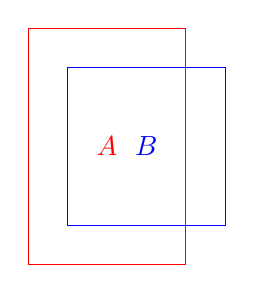
\begin{tikzpicture}
                    \draw[red] (0, 0) -- (2, 0) -- (2, 3) -- (0, 3) -- cycle;
                    \node[red] at (1, 1.5) {$A$};

                    \draw[blue] (0.5, 0.5) -- (2.5, 0.5) -- (2.5, 2.5) -- (0.5, 2.5) -- cycle;
                    \node[blue] at (1.5, 1.5) {$B$};
                \end{tikzpicture}
            \end{center}
            We consider the detection of the intersection over union (IoU) is above $0.5$;
            $$\text{IoU} = \frac{\red{A} \cap \blue{B}}{\red{A} \cup \blue{B}} > 0.5$$
            Another more complex piece of information we can extract is to perform \textbf{image segmentation}, allowing us to draw contours for each object.
            \subsubsection*{Applications}
                Computer vision is used in our lives daily;
                \begin{itemize}
                    \itemsep0em
                    \item \textbf{face detection}
                        \smallskip

                        This can be noticed in most camera applications on modern smartphones, when a small box is drawn around faces.
                        The algorithm first extracts \textbf{Haar} features from an image, and then determines (with these features) whether a region is a face or not.
                        \medskip

                        One example of these features is checking the contrast between the eyes and nose (horizontally); as the eyes tend to be quite dark in comparison.
                        Another contrast is checked, this time between your eyes, as the nose tends to be brighter.
                    \item \textbf{automatic number plate recognition}
                        \smallskip

                        Automated barriers in parking lots can read number plates in order to calculate how long a car stays.
                        Similarly, this can also be used to recognise building numbers, which is overlaid onto \textit{Google Maps}, allowing for a large database of street numbers to be built in an automated fashion.
                    \item \textbf{autonomous driving}
                    \item \textbf{image style transfer}
                        \smallskip

                        \textit{Choi et al. StarGAN: Unified Generative Adversarial Networks for Multi-Domain Image-to-Image Translation} - used for changing features on inputs.
                        Related to face motion capture (see \textit{Face2Face}).
                        Also see \textit{DeepFake}.
                    \item \textbf{Kinect}
                        \smallskip

                        Works by taking a depth image, segmenting it into body parts, locating key points and building a skeleton.
                    \item \textbf{design}
                        \smallskip

                        See \textit{OpenAI}'s \textit{DALL-E}, combining NLP and computer vision by generating images based on the concepts of words in a sentence.
                    \item \textbf{healthcare}
                        \smallskip

                        Medical image analysis can be used for disease diagnosis.
                        For example, identifying breast cancer lesions from mammograms.
                \end{itemize}
        \subsection*{Lecture 2 - Image Formation}
            An image, in RGB format, can be represented as pixels, each being three numbers.
            A digital image is formed from a lighting source being reflected into an optics sensor (eyes, cameras, etc).
            \subsubsection*{Light}
                A \textbf{point light source} originates from a single location in space, such as a small light bulb, or the sun.
                This can be described with three properties; location, intensity, and the spectrum.
                \medskip

                On the other hand, an \textbf{area light source} is more complex.
                For example, this could be a ceiling light; a rectangle of point lights.
            \subsubsection*{Reflectance}
                When light emitted from the source hits the surface of an object, it will be reflected.
                To describe this, we typically use the \textbf{bidirectional reflectance distribution function (BDRF)} to model this behaviour (where $\lambda$ is the wavelength, $L_r$ is the output power, and $E_i$ is the input power);
                $$f_r(\underbrace{\theta_i, \varphi_i}_\text{incident}, \underbrace{\theta_r, \varphi_r}_\text{reflected}, \lambda) = \dif{L_r}{E_i}$$
                While this is a very general model, it is very complex.
                \medskip

                As such, we can use \textbf{diffuse reflection}, where light is assumed to be scattered uniformly in all directions.
                This has a constant BRDF - this says that regardless of the incident or reflected directions, nor the wavelength, the power will be constant;
                $$f_r(\theta_i, \varphi_i, \theta_r, \varphi_r,, \lambda) = f_r(\lambda)$$
                \begin{center}
                    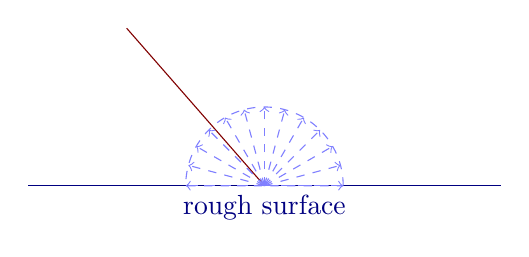
\begin{tikzpicture}
                        \draw[blue!50!black] (0, 0) edge[below] node{rough surface} (6, 0);
                        \draw[red!50!black] (1.25, 2) edge[->] (3, 0);
                        \draw[dashed, blue!50]
                        (4, 0) arc(0:180:1) -- cycle
                        (3, 0) edge[->] +(0:1)
                        (3, 0) edge[->] +(15:1)
                        (3, 0) edge[->] +(30:1)
                        (3, 0) edge[->] +(45:1)
                        (3, 0) edge[->] +(60:1)
                        (3, 0) edge[->] +(75:1)
                        (3, 0) edge[->] +(90:1)
                        (3, 0) edge[->] +(105:1)
                        (3, 0) edge[->] +(120:1)
                        (3, 0) edge[->] +(135:1)
                        (3, 0) edge[->] +(150:1)
                        (3, 0) edge[->] +(165:1)
                        (3, 0) edge[->] +(180:1);
                    \end{tikzpicture}
                \end{center}
                On the other hand, we can use \textbf{specular reflection} which performs reflections in a mirror-like fashion.
                The reflection and incident directions are symmetric with respect to the surface normal $\vec{n}$, such that $\theta_r = \theta_i$, with the same amount of power;
                \begin{center}
                    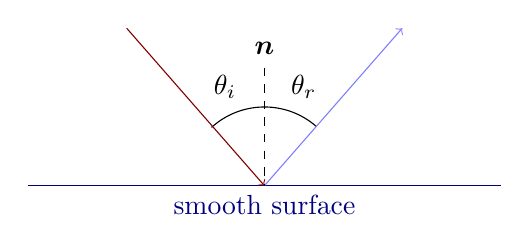
\begin{tikzpicture}
                        \draw (3, 0) ++(48.8:1) arc (48.8:132.2:1);
                        \draw[blue!50!black] (0, 0) edge[below] node{smooth surface} (6, 0);
                        \draw[red!50!black] (1.25, 2) edge[->] (3, 0);
                        \draw[blue!50] (4.75, 2) edge[<-] (3, 0);
                        \draw[dashed] (3, 1.5) -- (3, 0);

                        \node at (3, 1.75) {$\vec{n}$};
                        \node at (2.5, 1.25) {$\theta_i$};
                        \node at (3.5, 1.25) {$\theta_r$};
                    \end{tikzpicture}
                \end{center}
                While these two are the \textbf{ideal} cases, the majority of cases, we see a combination of both of those, as well as \textbf{ambient} illumination.
                Ambient illumination accounts for general illumination which could be complicated to model.
                For example, these could be repeated reflections between walls (which would be very difficult to calculate), and we instead assume that there is some light that exists in the 3D space representing the room.
                Another example could be a distance source, such as the sky (which has atmosphere).
                \medskip

                Combining these, we can use the \textbf{Phong} reflection model.
                This is an empirical model that describes how a surface reflects light as a combination of ambient, diffuse, and specular components.
            \subsubsection*{`Duality' with Computer Graphics}
                Using the game engine to produce example images is useful, as we are able to directly obtain the labels of objects from the engine itself, as well as visual output.
                As such, we can use these images as training for a model, since we also have an associated label map.
                This synthetic data is complementary to time-consuming manual annotations.
            \subsubsection*{Optics and Sensors}
                Both our eyes and cameras work in similar ways, with a lens governed by the thin lens equation, where $f$ denotes the focal length of the lens, $u$ denotes the distance from the subject to the lens, and $v$ denotes the distance from the lens to the image;
                $$\frac{1}{f} = \frac{1}{u} + \frac{1}{v}$$
                Our eyes work by light rays being focused by the cornea and lens onto the retina, where vision begins with two neural cells.
                The \textbf{cone} cells are responsible for colour vision, and function in bright light.
                On the other hand, the \textbf{rod} cells have little role in colour vision, but function in dim light.
                \medskip

                Humans have three types of cone cells (\textbf{trichromatic vision}), which have different response curves.
                The short cone cells respond to short wavelength lights (\violet{violet}, \blue{blue}), whereas the medium cone cells respond to medium wavelength lights (\textcolor{green}{green}), and long cone cells respond to long wavelength lights (\red{red}).
                Occasionally, there may be two cone cells, or four, which are referred to as \textbf{dichromacy} or \textbf{tetrachromacy} respectively.
                \medskip

                Note that colours are not objective physical properties of light or electromagnetic wave (which have a physical property of wavelength).
                Colour is a subjective feature, dependent on the visual perception of the observer.
                Since \textbf{rod} cells are more sensitive to light, they are the primary source of visual information at night.
                \medskip

                On the other hand, camera sensors have two common types;
                \begin{itemize}
                    \itemsep0em
                    \item \textbf{CCD} (charged-coupled device) \hfill often used in handheld cameras
                    \item \textbf{CMOS} (complementary metal-oxide semiconductor) \hfill used by most smartphone cameras
                \end{itemize}
                These sensors convert incoming light into electron charges, which are then read.
                \textbf{Bayer} filter arrays are a way to arrange RGB filters on sensors, half of which are green, and the remaining two quarters are red and blue.
                This mimics the human eyes, which are most sensitive to green light;
                \begin{center}
                    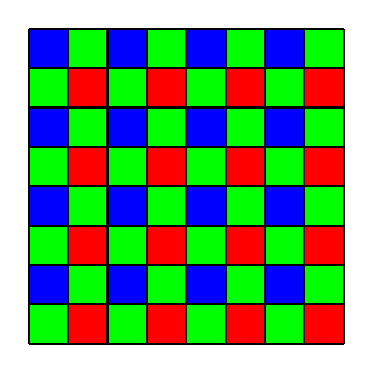
\begin{tikzpicture}[x=0.5cm, y=-0.5cm] % I should've just taken a screenshot, why do I keep doing this to myself
                        \foreach \i in {0,...,7} {
                            \foreach[evaluate={
                                \g=int(mod(\i + \j, 2);
                                \jm=int(mod(\j, 2))
                            }] \j in {0,...,7} {
                                \ifthenelse{\g = 1}
                                    {\def\col{green}}
                                    {\ifthenelse{\jm = 0}
                                        {\def\col{blue}}
                                        {\def\col{red}}}
                                \draw[fill=\col, draw=none] (\i, \j) -- (\i + 1, \j) -- (\i + 1, \j + 1) -- (\i, \j + 1) -- cycle;
                            }
                        }
                        \foreach \x in {0,...,8} {\draw[thick] (\x, 0) -- (\x, 8);}
                        \foreach \y in {0,...,8} {\draw[thick] (0, \y) -- (8, \y);}
                    \end{tikzpicture}
                \end{center}
                CMOS works by having sensors underneath each of these filtered portions, which can report an electrical signal.
                However, note that only one colour is available at each pixel (therefore the rest must be interpolated from the neighbours, by using bilinear interpolation; which simply averages the 4 neighbours).
                For example, consider the following pixel (denoted as a white cross);
                \begin{center}
                    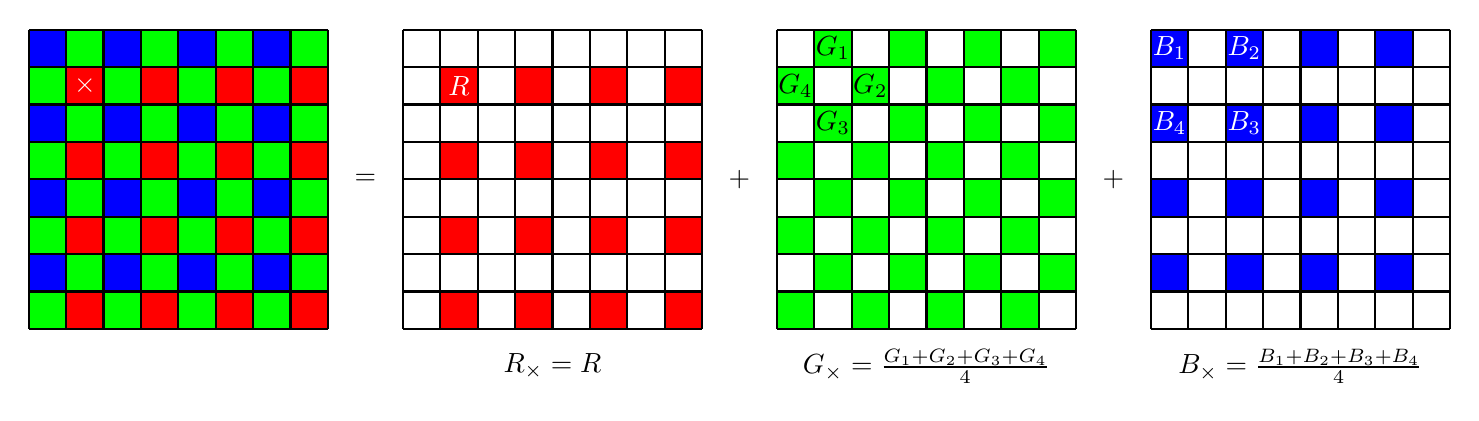
\begin{tikzpicture}[x=0.475cm, y=-0.475cm] % I should've just taken a screenshot, why do I keep doing this to myself
                        \begin{scope}[shift={(0, 0)}]
                            \foreach \i in {0,...,7} {
                                \foreach[evaluate={
                                    \g=int(mod(\i + \j, 2);
                                    \jm=int(mod(\j, 2))
                                }] \j in {0,...,7} {
                                    \ifthenelse{\g = 1}
                                        {\def\col{green}}
                                        {\ifthenelse{\jm = 0}
                                            {\def\col{blue}}
                                            {\def\col{red}}}
                                    \draw[fill=\col, draw=none] (\i, \j) -- (\i + 1, \j) -- (\i + 1, \j + 1) -- (\i, \j + 1) -- cycle;
                                }
                            }
                            \foreach \x in {0,...,8} {\draw[thick] (\x, 0) -- (\x, 8);}
                            \foreach \y in {0,...,8} {\draw[thick] (0, \y) -- (8, \y);}

                            \node[white] at (1.5, 1.5) {$\times$};
                        \end{scope}
                        \begin{scope}[shift={(10, 0)}]
                            \foreach \i in {0,...,7} {
                                \foreach[evaluate={
                                    \g=int(mod(\i + \j, 2);
                                    \jm=int(mod(\j, 2))
                                }] \j in {0,...,7} {
                                    \ifthenelse{\g = 1}
                                        {\def\col{white}}
                                        {\ifthenelse{\jm = 0}
                                            {\def\col{white}}
                                            {\def\col{red}}}
                                    \draw[fill=\col, draw=none] (\i, \j) -- (\i + 1, \j) -- (\i + 1, \j + 1) -- (\i, \j + 1) -- cycle;
                                }
                            }
                            \foreach \x in {0,...,8} {\draw[thick] (\x, 0) -- (\x, 8);}
                            \foreach \y in {0,...,8} {\draw[thick] (0, \y) -- (8, \y);}

                            \node[white] at (1.5, 1.5) {$R$};
                        \end{scope}
                        \begin{scope}[shift={(20, 0)}]
                            \foreach \i in {0,...,7} {
                                \foreach[evaluate={\g=int(mod(\i + \j, 2)}] \j in {0,...,7} {
                                    \ifthenelse{\g = 1}
                                        {\def\col{green}}
                                        {\def\col{white}}
                                    \draw[fill=\col, draw=none] (\i, \j) -- (\i + 1, \j) -- (\i + 1, \j + 1) -- (\i, \j + 1) -- cycle;
                                }
                            }
                            \foreach \x in {0,...,8} {\draw[thick] (\x, 0) -- (\x, 8);}
                            \foreach \y in {0,...,8} {\draw[thick] (0, \y) -- (8, \y);}

                            \node at (1.5, 0.5) {$G_1$};
                            \node at (2.5, 1.5) {$G_2$};
                            \node at (1.5, 2.5) {$G_3$};
                            \node at (0.5, 1.5) {$G_4$};
                        \end{scope}
                        \begin{scope}[shift={(30, 0)}]
                            \foreach \i in {0,...,7} {
                                \foreach[evaluate={
                                    \g=int(mod(\i + \j, 2);
                                    \jm=int(mod(\j, 2))
                                }] \j in {0,...,7} {
                                    \ifthenelse{\g = 1}
                                        {\def\col{white}}
                                        {\ifthenelse{\jm = 0}
                                            {\def\col{blue}}
                                            {\def\col{white}}}
                                    \draw[fill=\col, draw=none] (\i, \j) -- (\i + 1, \j) -- (\i + 1, \j + 1) -- (\i, \j + 1) -- cycle;
                                }
                            }
                            \foreach \x in {0,...,8} {\draw[thick] (\x, 0) -- (\x, 8);}
                            \foreach \y in {0,...,8} {\draw[thick] (0, \y) -- (8, \y);}

                            \node[white] at (0.5, 0.5) {$B_1$};
                            \node[white] at (2.5, 0.5) {$B_2$};
                            \node[white] at (2.5, 2.5) {$B_3$};
                            \node[white] at (0.5, 2.5) {$B_4$};
                        \end{scope}
                        \node at (9, 4) {$=$};
                        \node at (19, 4) {$+$};
                        \node at (29, 4) {$+$};

                        \node at (14, 9) {$R_\times = R$};
                        \node at (24, 9) {$G_\times = \frac{G_1 + G_2 + G_3 + G_4}{4}$};
                        \node at (34, 9) {$B_\times = \frac{B_1 + B_2 + B_3 + B_4}{4}$};
                    \end{tikzpicture}
                \end{center}
                Note that the use of different filters, and this interpolation, can lead to slightly different colours between cameras.
            \subsubsection*{Image Representation}
                The earliest colour space was described in 1931 by CIE, by performing a colour matching experiment.
                In this experiment, an observer attempts to match different levels of red, green, and blue lights to match a target light.
                This allows for colours to be represented in 3D space, as $(X, Y, Z)$, corresponding to the different levels.
                Colours can also be represented on a 2D plane, by normalising brightness;
                \begin{align*}
                    x & = \frac{X}{X + Y + Z} \\
                    y & = \frac{Y}{X + Y + Z} \\
                    z & = \frac{Z}{X + Y + Z} \\
                    & = 1 - x - y & \text{therefore redundant}
                \end{align*}
                Here $X, Y, Z$ are primary colours ($R, G, B$), and $x, y$ are chromacity / colour after removing brightness.
                This is much easier to draw.
                However, this colour space, also known as the \textbf{gamut} of human vision, was invented before computer screens.
                \medskip

                The sRGB (standard RGB) space was created by \textit{HP} and \textit{Microsoft} in 1996 for use on monitors, printers, and the internet.
                \begin{center}
                    \begin{tabular}{lcc}
                        sRGB definition & $x$ & $y$ \\
                        \hline
                        \red{red} & 0.64 & 0.33 \\
                        \textcolor{green}{green} & 0.30 & 0.60 \\
                        \blue{blue} & 0.15 & 0.06
                    \end{tabular}
                \end{center}
                This is represented by a triangle (which is a subset) in the gamut of human vision.
                As this is a subset, it cannot produce all the colours visible by the human eye.
                \medskip

                There are other colour spaces, such as HSV, CMYK, and so on.
                Note that CMYK is a \textbf{subtractive} colour model, starting from white, whereas RGB is an \textbf{additive} colour model, where we start from black.
                There can also be an alpha channel in RGB, which represents transparency.
                In a greyscale image, the three components are equal, hence only require one number.
            \subsubsection*{Quantisation}
                Note that this is covered in lecture 3.
                \medskip

                \textbf{Quantisation} maps a continuous signal to a discrete signal.
                The pictures from a camera are a continuous signal, but when it is stored on the camera, it is quantised to a discrete signal.
                Numerical errors can occur during this process, and the magnitude of the errors depends on the number of bits used (less error with more bits; 16 bits can store from 0 to 65535, compared to 8 bits storing from 0 to 255).
                \medskip

                Physically, an analog-to-digital convert (ADC) is used to perform the conversion.
                The energy of photons are converted into voltage, amplified, and then converted.
            \subsubsection*{Compression}
                In order to reduce the cost of storage to transmission, compression may be used.
                Lossy compression loses information after the compression (such as discrete cosine transform (DCT) in JPEG, often used for images or videos).
                However, lossless compression can also reduce the file size (less efficient compared to lossy), and is preferred for archival purposes or important imaging, where detail needs to be recovered.
        \subsection*{Lecture 3 - Image Filtering I}
            Note that in this course, most of the examples will be done on greyscale images, but can be applied to the channels individually.
            Some examples of filters include;
            \begin{itemize}
                \itemsep0em
                \item identity filter
                    \smallskip

                    Does nothing to the image.
                \item low-pass / smoothing (moving average, Gaussian)
                    \smallskip

                    Removes high-frequency signals, and keep low-frequency signals.
                \item high-pass / sharpening
                    \smallskip

                    Similar to the previous filter (keeps high-frequency signals, and removes low-frequency).
                \item denoise (median, non-local means, block-matching and 3D filtering)
            \end{itemize}
            \subsubsection*{Moving Average Filter}
                This is commonly used for 1D signal processing (time series), such as stocks, which can be quite noisy.
                To smooth out a noisy curve, it moves a window across the signal (and calculates the average value within the window) - the larger the window size, the smoother the result.
                \medskip

                In a two dimensional case, we can use a \textbf{filter kernel} (for example, with a $3 \times 3$ kernel);
                $$\frac{1}{9} \begin{bmatrix}
                    1 & 1 & 1 \\
                    1 & 1 & 1 \\
                    1 & 1 & 1
                \end{bmatrix}$$
                At each pixel, we apply the kernel centred at the pixel, and take the average of the pixels around it (and itself) to create a new output image.
                When we blur with a larger kernel, such as $7 \times 7$, we end up with a blurrier image.
                Note that the output image is smaller than the input image.
                We can pad the image with zeroes (anything outside of the picture is 0), or by mirroring the pixels (copying the boundary pixels).
                \medskip

                Consider an image of size $N \times N$, and a kernel size of $K \times K$.
                At each pixel, we perform $K^2$ multiplications (by the kernel weights), and then $K^2 - 1$ summations.
                This has to be done for each pixel, hence $N^2$ times.
                Therefore this results in $N^2 K^2$ multiplications and $N^2 (K^2 - 1)$ summations; giving a \textbf{complexity} of $O(N^2 K^2)$.
                However, we'd like to reduce this, if possible.
                \medskip

                If a big filter can be separated as two filters (\textbf{separable filter}) applied consecutively, we can perform the first operation, and then the second.
                An average in a 2D window can be done as an average across rows (horizontal), and then an average across columns (vertical);
                $$\begin{bmatrix}
                    \frac{1}{9} & \frac{1}{9} & \frac{1}{9} \\
                    \frac{1}{9} & \frac{1}{9} & \frac{1}{9} \\
                    \frac{1}{9} & \frac{1}{9} & \frac{1}{9}
                \end{bmatrix} = \begin{bmatrix}
                    \frac{1}{3} & \frac{1}{3} & \frac{1}{3}
                \end{bmatrix} * \begin{bmatrix}
                    \frac{1}{3} \\ \frac{1}{3} \\ \frac{1}{3}
                \end{bmatrix}$$
                Doing these two filters, we end up with an equivalent result to the original 2D filter.
                Note that $*$ is a convolution (see next lecture).
                \medskip

                Consider the complexity of separable filtering.
                The image size remains as $N \times N$, however we have two kernels, of $1 \times K$ and $K \times 1$ respectively.
                At each pixel we do $K$ multiplications followed by $K - 1$ summations.
                Again, this is done for $N^2$ pixels, and twice (once for each filter).
                Therefore, the total number of multiplications is $2N^2K$ multiplications and $2N^2(K - 1)$ summations.
                This is better, in contrast to the original complexity, as we have complexity of $O(N^2K)$ - which will make a difference for large $K$.
                \medskip

                A moving average filter removes high frequency signals (noise or sharpness), which results in a smooth but blurry image.
            \subsubsection*{Gaussian Filter}
                The kernel is a 2D Gaussian distribution;
                $$h(i, j) = \frac{1}{2 \pi \sigma^2} e^{-\frac{i^2 + j^2}{2 \sigma^2}}$$
                Here we have $i, j = 0, 0$ as the centre of the kernel.
                While the support is infinite, small values outside the range $[-k\sigma, k\sigma]$ can be ignored (very small values, such as $k=3$ or $k=4$).
                Note that $\sigma$ is a manually defined parameter.
                This is a separable filter, which is equivalent to two 1D Gaussian filters with the same $\sigma$, with one along the $x$-axis and the other along the $y$-axis;
                \begin{align*}
                    h(i, j) & = h_x(i) * h_y(j) \\
                    h_x(i) & = \frac{1}{\sqrt{2 \pi \sigma^2}} e^{-\frac{i^2}{2\sigma^2}}
                \end{align*}
            \subsubsection*{High-pass Filter}
                One design is to do the following;
                $$\underbrace{\begin{bmatrix}
                    0 & 0 & 0 \\
                    0 & 1 & 0 \\
                    0 & 0 & 0
                \end{bmatrix}}_\text{identity} + \underbrace{\left(\begin{bmatrix}
                    0 & 0 & 0 \\
                    0 & 1 & 0 \\
                    0 & 0 & 0
                \end{bmatrix} - \begin{bmatrix}
                    \frac{1}{9} & \frac{1}{9} & \frac{1}{9} \\
                    \frac{1}{9} & \frac{1}{9} & \frac{1}{9} \\
                    \frac{1}{9} & \frac{1}{9} & \frac{1}{9}
                \end{bmatrix}\right)}_\text{high-frequency} = \begin{bmatrix}
                    -\frac{1}{9} & -\frac{1}{9} & -\frac{1}{9} \\
                    -\frac{1}{9} & \frac{17}{9} & -\frac{1}{9} \\
                    -\frac{1}{9} & -\frac{1}{9} & -\frac{1}{9}
                \end{bmatrix}$$
                We can add a high frequency signal to the identity, in order to enhance it.
            \subsubsection*{Median Filter}
                This is a non-linear filter (not performing an average calculation by multiplication).
                This moves a sliding window, and replaces the centre pixel with the median value in the window - this is not a linear equation.
        \subsubsection*{Lecture 4 - Image Filtering II}
            \subsubsection*{Mathematical Description}
                Consider a simple filter, of size 3, in 1D.
                With an input $f$, and an output $g$, it can be written as the weighted average in a window;
                $$g[n] = \frac{1}{3} f[n - 1] + \frac{1}{3} f[n] + \frac{1}{3} f[n + 1]$$
                In general, filtering takes in an input signal $f$, processes it and generates an output signal $g$.
                A filter is a device (or process) that removes unwanted components or features from a signal (keeps / enhances wanted filters).
                \medskip

                In order to mathematically describe a filter, we need the concept of \textbf{impulse response}; the output of a  filter when the input is an \textbf{impulse signal} (only have a signal at a single time point);
                \begin{center}
                    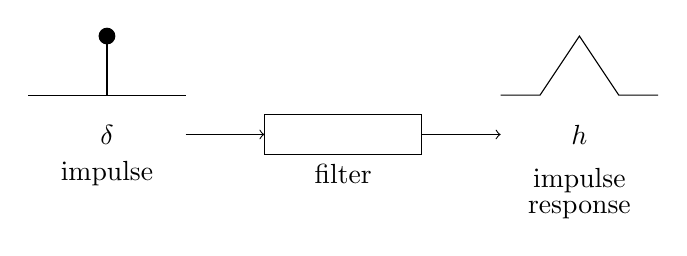
\begin{tikzpicture}
                        \begin{scope}
                            \draw (0, 0) -- (2, 0);
                            \draw (1, 0) -- (1, 0.75);
                            \node[rbtb] at (1, 0.75) {};
                            \node at (1, -0.5) {$\delta$};
                            \node at (1, -1) {impulse};
                        \end{scope}
                        \draw (2, -0.5) edge[->] (3, -0.5);
                        \draw (5, -0.5) edge[->] (6, -0.5);
                        \draw (3, -0.25) -- (5, -0.25) -- (5, -0.75) -- (3, -0.75) -- cycle;
                        \node at (4, -1) {filter};
                        \begin{scope}[shift={(6, 0)}]
                            \draw (0, 0) -- (0.5, 0) -- (1, 0.75) -- (1.5, 0) -- (2, 0);
                            \node at (1, -0.5) {$h$};
                            \node at (1, -1.25) {\shortstack{impulse\\response}};
                        \end{scope}
                    \end{tikzpicture}
                \end{center}
                For a continuous signal, we treat an impulse as a Dirac delta function $\delta(x)$, whereas for a discrete signal, we treat an impulse as a Kronecker delta function $\delta[i]$;
                \begin{align*}
                    \delta(x) & = \begin{cases}
                        \infty & \text{if } x = 0 \\
                        0 & \text{otherwise}
                    \end{cases} \\
                    \defint{-\infty}{\infty}{\delta(x)}{x} & = 1 \\
                    \delta[i] & = \begin{cases}
                        1 & \text{if } i = 0 \\
                        0 & \text{otherwise}
                    \end{cases}
                \end{align*}
                The impulse response $h$ completely characterises a \textbf{linear time-invariant} filter.
                Note that we can consider a filter as time-invariant if, by shifting the input signal some number of time steps $k$, the output signal will remain the same (shape and values) but shifted by the \textbf{same} number of time steps.
                For example;
                \begin{itemize}
                    \itemsep0em
                    \item $g[n] = 10 \cdot f[n]$ is time-invariant and amplifies the input by a constant
                    \item $g[n] = n \cdot f[n]$ is \textbf{not} time-invariant since the amount it amplifies the input depends on the time step $n$
                \end{itemize}
                As long as we know $h$, and have an input $x$, we can calculate the output signal $y$.
                Since it uniquely describes a filter, we often denote a filter by its impulse response function $h$.
                \medskip

                Additionally, a filter can be \textbf{linear}.
                If it is a linear system, when two input signals are combined linearly, their outputs will also be combined linearly.
                Let $f_1[n]$ lead to an output $g_1[n]$, and $f_2[n]$ to $g_2[n]$.
                $$\text{output}(\alpha f_1[n] + \beta f_2[n]) = \alpha g_1[n] + \beta g_2[n]$$
            \subsubsection*{Convolution}
                Most of the filters we've previously covered are linear time-invariant.
                Since $h$ characterises how the system works (as it is linear time-invariant), it's possible for the output $g$ to be described as the \textbf{convolution} between an input $f$ and impulse response $h$;
                $$g[n] = f[n] * h[n]$$
                \medskip

                We can describe an input signal $f[n]$ as the following, where each time step is a constant multiplied by a spike;
                $$f[n] = f[0]\delta[n] + f[1]\delta[n - 1] + f[2]\delta[n - 2] + f[3]\delta[n - 3] + \dots$$
                However, since we know the output of $\delta[n]$ is $h[n]$, we can write the output as;
                $$g[n] = f[0]h[n] + f[1]h[n - 1] + f[2]h[n - 2] + f[3]h[n - 3] + \dots$$
                The output mathematical operation is defined as a convolution, where a signal $f$ and a filter with impulse response / convolution kernel $h$ is defined as;
                $$g[n] = f[n] * h[n] = \summation{m = -\infty}{\infty} f[m]h[n - m]$$
                The continuous form (previously we have only considered the discrete form);
                $$g(t) = f(t) * h(t) = \defint{-\infty}{\infty}{f(\tau) h(t - \tau)}{\tau}$$
                Focusing on the discrete case, we notice the following (when we replace $m$ with $n - m$);
                $$\summation{m = -\infty}{\infty} f[m]h[n - m] = \summation{m = -\infty}{\infty} f[n - m]h[m]$$
                This shows that the convolution of $f$ and $h$ is equivalent to the convolution of $h$ and $f$ (commutativity);
                $$f[n] * h[n] = h[n] * f[n]$$
                By expanding the equations, we can also show that convolution satisfies associativity, such that;
                $$f * (g * h) = (f * g) * h$$
                We also have distributivity;
                $$f * (g + h) = (f * g) + (f * h)$$
                And also differentiation;
                $$\dif{}{x}(f * g) = \dif{f}{x} * g = f * \dif{g}{x}$$
                With a more concrete example, we can visualise it as follows (this is the moving average of size 3);
                \begin{center}
                    \begin{tikzpicture}
                        \begin{scope}[shift={(0, 1.5)}]
                            \draw (1, 0) -- (4, 0) -- (4, -1) -- (1, -1) -- cycle;
                            \foreach \i in {1,...,2} {
                                \draw (\i + 1, 0) -- (\i + 1, -1);
                            }
                            \node at (1.5, -0.5) {\tiny $h[1]$};
                            \node at (2.5, -0.5) {\tiny $h[0]$};
                            \node at (3.5, -0.5) {\tiny $h[-1]$};
                        \end{scope}

                        \draw (0, 0) -- (6, 0) -- (6, -1) -- (0, -1) -- cycle;
                        \foreach \i in {1,...,5} {
                            \draw (\i, 0) -- (\i, -1);
                        }
                        \node at (1.5, -0.5) {\tiny$f[n - 1]$};
                        \node at (2.5, -0.5) {\tiny$f[n]$};
                        \node at (3.5, -0.5) {\tiny$f[n + 1]$};

                        \draw (8, 0) -- (14, 0) -- (14, -1) -- (8, -1) -- cycle;
                        \foreach \i in {1,...,5} {
                            \draw (\i + 8, 0) -- (\i + 8, -1);
                        }
                        \node at (10.5, -0.5) {\tiny$g[n]$};
                    \end{tikzpicture}
                \end{center}
                In our case, we have the kernel $h[n]$, and the values;
                \begin{align*}
                    h[-1] & = \frac{1}{3} \\
                    h[0] & = \frac{1}{3} \\
                    h[1] & = \frac{1}{3} \\
                    h[n] & = \begin{bmatrix}
                        \frac{1}{3}, & \frac{1}{3}, & \frac{1}{3}
                    \end{bmatrix}
                \end{align*}
                This can be expanded into the 2D case, which is used for image filtering;
                $$g[m, n] = f[m, n] * h[m, n] = \summation{i = -\infty}{\infty} \summation{j = -\infty}{\infty} f[i, j] h[m - i, n - j]$$
                This can also be written as the following, replacing $m - i, n - j$ by $i, j$;
                $$g[m, n] = \summation{i = -\infty}{\infty} \summation{j = -\infty}{\infty} f[m - i, n - j] h[i, j]$$
                By using the property of associativity, if a big filter (call it $f_b$) can be written as the convolution of $g$ and $h$ (smaller filters), we can first convolve $f$ with $g$, then with $h$ - this is used for separable filtering;
                $$f * f_b = f * (g * h) = (f * g) * h$$
                For example (note that we have padded zeroes, but in code we do not need that);
                $$\underbrace{\begin{bmatrix}
                    \frac{1}{9} & \frac{1}{9} & \frac{1}{9} \\
                    \frac{1}{9} & \frac{1}{9} & \frac{1}{9} \\
                    \frac{1}{9} & \frac{1}{9} & \frac{1}{9}
                \end{bmatrix}}_{f_b} = \underbrace{\begin{bmatrix}
                    \textcolor{black!33}{0} & \textcolor{black!33}{0} & \textcolor{black!33}{0} \\
                    \frac{1}{3} & \frac{1}{3} & \frac{1}{3} \\
                    \textcolor{black!33}{0} & \textcolor{black!33}{0} & \textcolor{black!33}{0}
                \end{bmatrix}}_{g} * \underbrace{\begin{bmatrix}
                    \textcolor{black!33}{0} & \frac{1}{3} & \textcolor{black!33}{0} \\
                    \textcolor{black!33}{0} & \frac{1}{3} & \textcolor{black!33}{0} \\
                    \textcolor{black!33}{0} & \frac{1}{3} & \textcolor{black!33}{0}
                \end{bmatrix}}_{h}$$
        \subsection*{Lecture 5 - Edge Detection I}
            \subsubsection*{Importance of Edges}
                In computer vision an edge refers to lines where image brightness changes sharply with discontinuities.
                This may be due to different reasons such as discontinuities in colour, depth, surface normals, etc.
                Edges capture important properties of what we see in the world, and they are important features for image analysis (for example, we first capture edges, then facial features, and so on).
                \textit{Hubel} and \textit{Wiesel} performed vision experiments in 1959, finding that neuron cells in the primary visual cortex are orientation selective, responding strongly to lines or edges of a particular orientation.
                Humans can also read images even if reduced to simple line drawings.
                Edges are also heavily used in convolutional networks, with the first layer tending to learn edges, with the later layers learning increasingly complex patterns.
            \subsubsection*{Detection}
                An image can be considered as a function of pixel positions (consider plotting the image on the $x-y$ axes, and having the $z$ axis denote intensity).
                Mathematically, derivatives characterise function discontinuities, which can be used to help edge detection.
                For a continuous function, the derivative is;
                $$f^\prime(x) = \limit{h}{0} \frac{f(x + h) - f(x)}{h}$$
                On the other hand, for a discrete function (finite difference);
                $$\underbrace{f^\prime[x] = f[x + 1] - f[x]}_\text{forward difference} \ \ \ \ \ \underbrace{f^\prime[x] = f[x] - f[x - 1]}_\text{backward difference} \ \ \ \ \ \underbrace{f^\prime[x] = \frac{f[x + 1] - f[x - 1]}{2}}_\text{central difference}$$
                Notice that these can also be performed with convolutions, using the following kernels;
                $$\underbrace{h = [1, -1, 0]}_\text{forward difference} \ \ \ \ \ \ \ \ \ \ \underbrace{h = [0, 1, -1]}_\text{backward difference} \ \ \ \ \ \ \ \ \ \  \underbrace{h = [1, 0, -1]}_\text{central difference}$$
            \subsubsection*{Prewitt and Sobel Filters}
                The Prewitt filters, along the $x$-axis (horizontal direction) and along the $y$-axis (vertical direction) are as follows;
                \begin{center}
                    \hfill
                    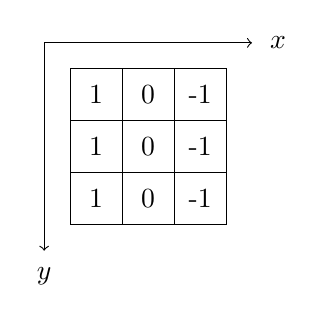
\begin{tikzpicture}[x=0.66cm, y=0.66cm]
                        \draw
                        (-0.5, 3.5) edge[->] (3.5, 3.5)
                        (-0.5, 3.5) edge[->] (-0.5, -0.5);
                        \node at (4, 3.5) {$x$};
                        \node at (-0.5, -1) {$y$};
                        \draw
                        (0, 0) -- (3, 0) -- (3, 3) -- (0, 3) -- cycle
                        (0, 1) -- (3, 1)
                        (0, 2) -- (3, 2)
                        (1, 0) -- (1, 3)
                        (2, 0) -- (2, 3);
                        \node at (0.5, 0.5) {1};
                        \node at (0.5, 1.5) {1};
                        \node at (0.5, 2.5) {1};
                        \node at (1.5, 0.5) {0};
                        \node at (1.5, 1.5) {0};
                        \node at (1.5, 2.5) {0};
                        \node at (2.5, 0.5) {-1};
                        \node at (2.5, 1.5) {-1};
                        \node at (2.5, 2.5) {-1};
                    \end{tikzpicture}
                    \hfill
                    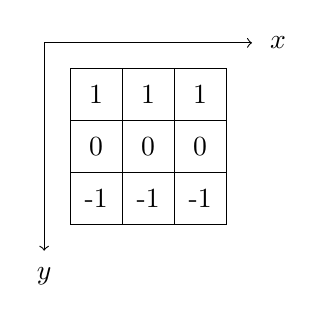
\begin{tikzpicture}[x=0.66cm, y=0.66cm]
                        \draw
                        (-0.5, 3.5) edge[->] (3.5, 3.5)
                        (-0.5, 3.5) edge[->] (-0.5, -0.5);
                        \node at (4, 3.5) {$x$};
                        \node at (-0.5, -1) {$y$};
                        \draw
                        (0, 0) -- (3, 0) -- (3, 3) -- (0, 3) -- cycle
                        (0, 1) -- (3, 1)
                        (0, 2) -- (3, 2)
                        (1, 0) -- (1, 3)
                        (2, 0) -- (2, 3);
                        \node at (0.5, 0.5) {-1};
                        \node at (0.5, 1.5) {0};
                        \node at (0.5, 2.5) {1};
                        \node at (1.5, 0.5) {-1};
                        \node at (1.5, 1.5) {0};
                        \node at (1.5, 2.5) {1};
                        \node at (2.5, 0.5) {-1};
                        \node at (2.5, 1.5) {0};
                        \node at (2.5, 2.5) {1};
                    \end{tikzpicture}
                    \hfill \phantom{}
                \end{center}
                Note that the Prewitt filter is a separable filter ([1] - moving average for smoothing);
                $$\underbrace{\begin{bmatrix}
                    1 & 0 & -1 \\
                    1 & 0 & -1 \\
                    1 & 0 & -1
                \end{bmatrix}}_\text{Prewitt filter} = \underbrace{\begin{bmatrix}
                    \textcolor{black!33}{0} & 1 & \textcolor{black!33}{0} \\
                    \textcolor{black!33}{0} & 1 & \textcolor{black!33}{0} \\
                    \textcolor{black!33}{0} & 1 & \textcolor{black!33}{0}
                \end{bmatrix}}_\text{[1]} * \underbrace{\begin{bmatrix}
                    \textcolor{black!33}{0} & \textcolor{black!33}{0} & \textcolor{black!33}{0} \\
                    1 & 0 & -1 \\
                    \textcolor{black!33}{0} & \textcolor{black!33}{0} & \textcolor{black!33}{0}
                \end{bmatrix}}_\text{finite difference}$$
                The Sobel filter is quite similar to the Prewitt filter;
                \begin{center}
                    \hfill
                    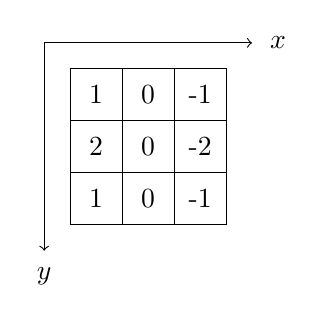
\begin{tikzpicture}[x=0.66cm, y=0.66cm]
                        \draw
                        (-0.5, 3.5) edge[->] (3.5, 3.5)
                        (-0.5, 3.5) edge[->] (-0.5, -0.5);
                        \node at (4, 3.5) {$x$};
                        \node at (-0.5, -1) {$y$};
                        \draw
                        (0, 0) -- (3, 0) -- (3, 3) -- (0, 3) -- cycle
                        (0, 1) -- (3, 1)
                        (0, 2) -- (3, 2)
                        (1, 0) -- (1, 3)
                        (2, 0) -- (2, 3);
                        \node at (0.5, 0.5) {1};
                        \node at (0.5, 1.5) {2};
                        \node at (0.5, 2.5) {1};
                        \node at (1.5, 0.5) {0};
                        \node at (1.5, 1.5) {0};
                        \node at (1.5, 2.5) {0};
                        \node at (2.5, 0.5) {-1};
                        \node at (2.5, 1.5) {-2};
                        \node at (2.5, 2.5) {-1};
                    \end{tikzpicture}
                    \hfill
                    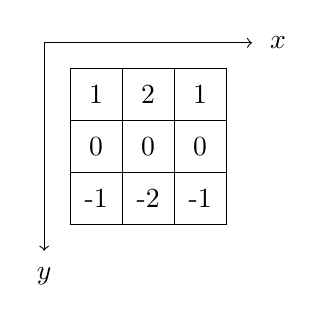
\begin{tikzpicture}[x=0.66cm, y=0.66cm]
                        \draw
                        (-0.5, 3.5) edge[->] (3.5, 3.5)
                        (-0.5, 3.5) edge[->] (-0.5, -0.5);
                        \node at (4, 3.5) {$x$};
                        \node at (-0.5, -1) {$y$};
                        \draw
                        (0, 0) -- (3, 0) -- (3, 3) -- (0, 3) -- cycle
                        (0, 1) -- (3, 1)
                        (0, 2) -- (3, 2)
                        (1, 0) -- (1, 3)
                        (2, 0) -- (2, 3);
                        \node at (0.5, 0.5) {-1};
                        \node at (0.5, 1.5) {0};
                        \node at (0.5, 2.5) {1};
                        \node at (1.5, 0.5) {-2};
                        \node at (1.5, 1.5) {0};
                        \node at (1.5, 2.5) {2};
                        \node at (2.5, 0.5) {-1};
                        \node at (2.5, 1.5) {0};
                        \node at (2.5, 2.5) {1};
                    \end{tikzpicture}
                    \hfill \phantom{}
                \end{center}
                Note that the Sobel filter is also a separable filter;
                $$\underbrace{\begin{bmatrix}
                    1 & 0 & -1 \\
                    2 & 0 & -2 \\
                    1 & 0 & -1
                \end{bmatrix}}_\text{Sobel filter} = \underbrace{\begin{bmatrix}
                    \textcolor{black!33}{0} & 1 & \textcolor{black!33}{0} \\
                    \textcolor{black!33}{0} & 2 & \textcolor{black!33}{0} \\
                    \textcolor{black!33}{0} & 1 & \textcolor{black!33}{0}
                \end{bmatrix}}_\text{smoothing} * \underbrace{\begin{bmatrix}
                    \textcolor{black!33}{0} & \textcolor{black!33}{0} & \textcolor{black!33}{0} \\
                    1 & 0 & -1 \\
                    \textcolor{black!33}{0} & \textcolor{black!33}{0} & \textcolor{black!33}{0}
                \end{bmatrix}}_\text{finite difference}$$
                Note that the outputs of the filters are different, with the horizontal filter detecting changes in the horizontal direction; describing discontinuity along the $x$-axis (leading to vertical lines).
                These can be combined to describe two properties of edges; the magnitude and the orientation.
                \begin{align*}
                    g_x & = f * h_x & \text{derivative along $x$-axis} \\
                    g_y & = f * h_y & \text{derivative along $y$-axis} \\
                    g & = \sqrt{g_x^2 + g_y^2} & \text{magnitude of the gradient} \\
                    \theta & = \mathrm{arctan2}(g_y, g_x) & \text{angle of the gradient}
                \end{align*}
            \subsubsection*{Derivative of Gaussian}
                Note that in both the filters above, there is some smoothing as derivatives are sensitive to noise (therefore the smoothing kernel helps to suppress noise).
                The Prewitt filters use the mean average kernel, whereas Sobel filters use the kernel $[1, 2, 1]$.
                Another option is to use the Gaussian kernel for smoothing, before calculating derivatives;
                $$h[x] = \frac{1}{\sqrt{2 \pi} \sigma}e^{-\frac{x^2}{2\sigma^2}}$$
                \medskip

                The derivative of Gaussian filter is an operation, performing Gaussian smoothing, before taking the derivative.
                However, recalling the rules for the differentiation of convolution, we have $f$ (input signal) convolved with the derivative of the Gaussian kernel;
                \begin{align*}
                    \dif{}{x}(f * h) & = f * \dif{h}{x} \\
                    & = f * \frac{-x}{\sqrt{2 \pi} \sigma^3} e^{-\frac{x^2}{2\sigma^2}}
                \end{align*}
                In the 2D case, the Gaussian filter is as follows;
                $$h[x, y] = \frac{1}{2 \pi \sigma^2}e^{-\frac{x^2 + y^2}{2 \sigma^2}}$$
                However, it is a separable filter (and therefore can be sped up) equivalent to the convolution of two 1D Gaussian filters.
                Notice there's a parameter $\sigma$ in the derivative of Gaussian.
                With a small $\sigma$, there is more detail in the magnitude map; on the other hand, a large $\sigma$ value suppresses noise and results in a smoother derivative.
                As such, different $\sigma$ values help to find edges at different scales.
        \subsection*{Lecture 6 - Edge Detection II}
            \subsubsection*{Canny Edge Detection}
                The results of the filters from the previous lectures (gradient magnitude map) have values ranging from black to white.
                However, we want either a 0 or 1 (black or white) - a \textbf{binary edge map}.
                \medskip

                There should be good detection; a low probability of failing too mark real edge points and low probability of falsely marking non-edge points.
                In addition, there should be good localisation - the points marked as edges should be as close as possible to the centre of the edge.
                Finally, there should only be a single response to a single edge.
                \medskip

                Canny edge detection is done in the following steps;
                \begin{enumerate}[1.]
                    \itemsep0em
                    \item perform Gaussian filtering to suppress noise
                        \smallskip

                        The choice of $\sigma$ depends on the type of edge we desire at the end.
                        If we want large edges (such as buildings), $\sigma$ should be set to a large value (such as 7).
                        However, if we want to pay attention to fine features, $\sigma$ can be set to a small value.
                    \item calculate gradient magnitudes and directions
                    \item apply non-maximum suppression (NMS) to get a single response for each edge
                        \smallskip

                        Non-maximum suppression aims to get a single response for each edge, by using the idea that the edge occurs where the gradient magnitude is maximum at the centre of the edge.
                        \begin{center}
                            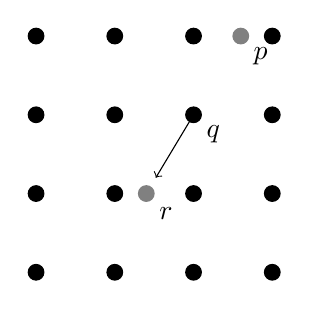
\begin{tikzpicture}
                                \foreach \x in {0,...,3} {
                                    \foreach \y in {0,...,3} {
                                        \node[rbtb] at (\x, \y) {};
                                    }
                                }
                                \node[inner sep=2pt, circle, draw=black!50, fill=black!50] at (2.6, 3) {};
                                \node[inner sep=2pt, circle, draw=black!50, fill=black!50] at (1.4, 1) {};
                                \node at (2.25, 1.75) {$q$};
                                \node at (2.85, 2.75) {$p$};
                                \node at (1.65, 0.75) {$r$};
                                \begin{scope}[shift={(2, 2)}, scale={0.8}]
                                    \draw (0, 0) edge[->] (-0.6, -1);
                                \end{scope}
                            \end{tikzpicture}
                        \end{center}
                        Compare the magnitude at $q$ with the magnitudes of $p$ and $r$, both along the gradient direction (in opposite directions).
                        If $q$ is the local maximum (larger than both $p$ and $r$), we keep the magnitude at pixel $q$.
                        $$M(x, y) = \begin{cases}
                            M(x, y) & \text{if local maximum} \\
                            0 & \text{otherwise}
                        \end{cases}$$
                        However, notice that there may be issues with $p$ and $r$ not being at exact pixel locations.
                        For example, using pixel $r$ (not at an integer position), we can perform interpolation.
                        It's possible to use linear interpolation (weighted by distance), or a simpler algorithm such as nearest neighbour interpolation (better performance).
                        Note that different interpolation algorithms will lead to different outcomes.
                        Another approach is to round the gradient direction into 8 possible angles, in steps of $45^\circ$ in the range $[0^\circ, 315^\circ]$, allowing us to check only along those directions to give exact pixels (intuitively quite similar to nearest neighbour).
                        \medskip

                        After NMS, there are fewer points with bright values.
                    \item perform hysteresis thresholding to find potential edges
                        \smallskip

                        Many pixels that are local maxima may still have very low magnitudes; however we only want edges with high magnitudes.
                        A simple thresholding would be to convert an intensity image to a binary image with a threshold $t$;
                        $$\text{binary}(x, y) = \begin{cases}
                            1 & \text{if } I(x, y) \geq t \\
                            0 & \text{otherwise}
                        \end{cases}$$
                        On the other hand, hysteresis thresholding defines two thresholds $t_\text{low}$ and $t_\text{high}$.
                        If the magnitude is $\geq t_\text{high}$, it is accepted as an edge pixel, and if it is $< t_\text{low}$, it is rejected.
                        However, if we have a value between the thresholds, we have a \textbf{weak edge} (which may or may not be an edge).
                        If it is connected to existing edge pixels, it is accepted, whereas if it is not connected (adjacent to one strong edge) to an existing edge, it will be rejected.
                \end{enumerate}
                The initial goals are satisfied as follows;
                \begin{itemize}
                    \itemsep0em
                    \item \textbf{good detection}
                        \smallskip

                        False positives are reduced by using Gaussian smoothing to suppress noise.
                        On the other hand, false negatives are reduced by using hysteresis thresholding to find weak edges.
                    \item \textbf{good localisation}
                        \smallskip

                        NMS finds locations based on gradient magnitude and direction.
                    \item \textbf{single response} \hfill also done with NMS
                \end{itemize}
            \subsubsection*{Learning-based Edge Detection}
                Decades of effort have been made to improve detection accuracy.
                This includes using richer features such as colour and texture, enforcing smoother, as well as using machine learning (by learning mapping from an image to edge directly from data).
                \medskip

                This machine learning algorithm assumes paired data (images $x$ and manually defined edge maps $y$).
                The problem finds a model (with model parameters $\theta$) that maps $x$ to $y$, such that $y = f(x\ |\ \theta)$.
                This differs from Canny edge detector, as our example integrates from multiple scales (fine-scale edges) with coarse-scale edges to form a final output.
                On the other hand, Canny edge detector uses a single scale for edge detection, controlled by a single parameter $\sigma$.
                \medskip

                An application for learning-based edge detection is to learn a mapping from a rough sketch to a simplified sketch.
                However, this isn't just an edge detection problem since it cannot be solved using NMS; when this is done by humans, a high-level understanding about the sketch is required.
            \subsubsection*{Conclusion}
                Edge detection is a fundamental problem in image processing and computer vision; aiming to identify where discontinuities occur, or identifying points that are edges.
                Two solutions are proposed;
                \begin{itemize}
                    \itemsep0em
                    \item if we know the explicit criteria, we can implement computational criteria
                    \item otherwise, we can collect data pairs representing what we want to achieve and train a machine learning model
                \end{itemize}
                Edges provide important low-level features both human vision and computer vision for understanding images.
                These algorithms provide ideas for other detection algorithms.
                \medskip

                We can also go in the other direction, taking edges to images.
                This aims to train a model that generates an image that looks close to real images, from edges.
                A model $G$ (generator) learns the mapping from edge to image.
                For example, we take an edge image $x$ to $G(x)$ (an image).
                A discriminator $d$ then attempts to assess whether the image is real or fake (GAN).
        \subsection*{Lecture 7 - Hough Transform}
            In the last lecture, we covered edge detection (1 for edge pixel, 0 for background).
            If we know these edges form some shape (such as a line), we want to obtain a parametric representation.
            \subsubsection*{Line Parameterisation}
                A line can be represented by two parameters (e.g. $m$ (slope) and $b$ ($y$-intercept)), which is much more efficient than a lot of edge points;
                \begin{itemize}
                    \itemsep0em
                    \item slope intercept form \hfill $m$ (slope) and $b$ ($y$-intercept)
                        $$y = mx + b$$
                    \item double intercept form \hfill $(a, 0)$ and $(0, b)$ are on the line
                        $$\frac{x}{a} + \frac{y}{b} = 1$$
                    \item normal form \hfill $\theta$ is angle and $\rho$ is distance
                        $$x\cos(\theta) + y\sin(\theta) = \rho$$
                \end{itemize}
            \subsubsection*{Hough Transform}
                Hough transform transforms from image space (edge map) to parameter space (two parameters of a line).
                The output is a parametric model, from a n input of edge points.
                Each edge point `votes' for possible models in the parameter space.
                One way is to fit a line model $(m, b)$ to the edge points $(x_1, y_1), (x_2, y_2), \dots$;
                $$\min_{m, b} \summation{i}{} (y_i - \underbrace{(mx_i + b)}_{\hat{y}})^2$$
                For the Hough transform we will use the slope intercept form.
                $$y = mx + b \Leftrightarrow b = y - mx$$
                Assume we have the edge points $(x_1, y_1), \dots$, each point will vote for a line model in the parameter space; for example, the first point votes for;
                $$b = y_1 - mx_1$$
                This can be seen graphically as the following (image space on the left, parameter space ($b = y - mx$) on the right);
                \begin{center}
                    \hfill
                    \begin{tikzpicture}
                        \begin{axis}[
                            axis on top=true,
                            axis line style=thick,
                            domain=-4:4, samples=9,
                            axis lines=middle, xlabel=$x$, ylabel=$y$,
                            height=8cm, width=8cm,
                            enlargelimits=false,
                            xtick={-4,-3,...,4},
                            ytick={-4,-3,...,4},
                            xmin=-4, xmax=4,
                            ymin=-4, ymax=4
                        ]
                            \node[label={45:{\tiny(3,3)}}, circle, fill=red, inner sep=2pt] at (axis cs:3,3) {};
                            \node[label={45:{\tiny(1,1)}}, circle, fill=green, inner sep=2pt] at (axis cs:1,1) {};
                            \node[label={135:{\tiny(-2,-2)}}, circle, fill=blue, inner sep=2pt] at (axis cs:-2,-2) {};
                        \end{axis}
                    \end{tikzpicture}
                    \hfill
                    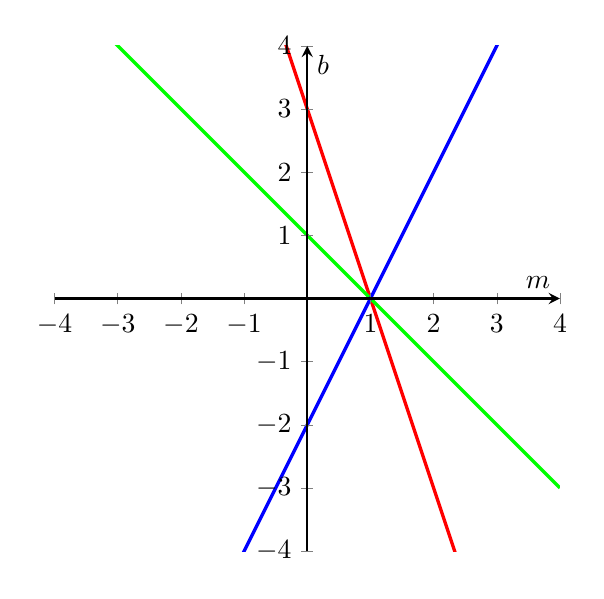
\begin{tikzpicture}
                        \begin{axis}[
                            axis on top=true,
                            axis line style=thick,
                            domain=-4:4, samples=9,
                            axis lines=middle, xlabel=$m$, ylabel=$b$,
                            height=8cm, width=8cm,
                            enlargelimits=false,
                            xtick={-4,-3,...,4},
                            ytick={-4,-3,...,4},
                            xmin=-4, xmax=4,
                            ymin=-4, ymax=4
                        ]
                            \addplot[very thick, red] {3 - 3*\x};
                            \addplot[very thick, green] {1 - \x};
                            \addplot[very thick, blue] {-2 + 2*\x};
                        \end{axis}
                    \end{tikzpicture}
                    \hfill \phantom{}
                \end{center}
                The intersection will get 3 votes, the other points on the line get 1 vote each, and the empty spaces get 0 votes.
                This gives a result of $m = 1$ and $b = 0$, thus we get the line $y = x$.
                However, in practice this is divided into two dimensional bins, with each point incrementing the vote by 1 in one of the bins.
                One problem is that the parameter space is too large for $m$ and $b$ (both are infinite).
                \medskip

                The solution to this is to use the normal form.
                While $\rho$ can still be infinite (in theory, however we can actually limit this to the image size in practice), we have $\theta \in [0, \pi)$.
                The transform from the image space to the parameter space ($x\cos(\theta) + y\sin(\theta) = \rho$) will however look different;
                \begin{center}
                    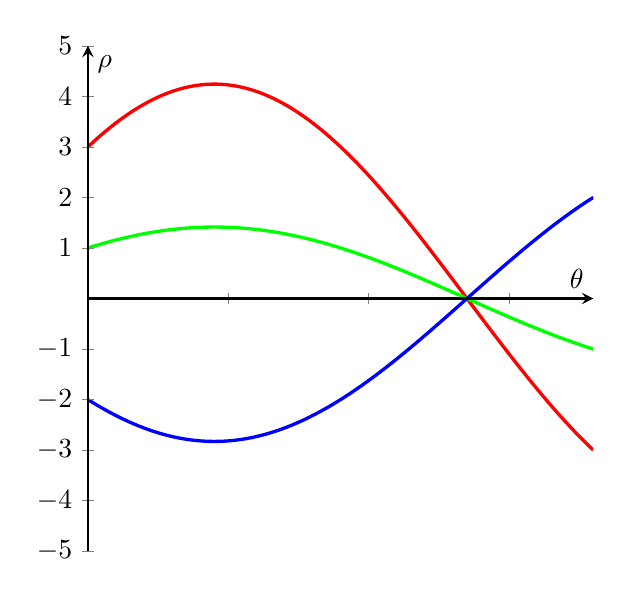
\begin{tikzpicture}
                        \begin{axis}[
                            axis on top=true,
                            axis line style=thick,
                            domain=0:180, samples=90,
                            axis lines=middle, xlabel=$\theta$, ylabel=$\rho$,
                            height=8cm, width=8cm,
                            enlargelimits=false,
                            xticklabels={,,},
                            ytick={-5,-4,...,5},
                            xmin=0, xmax=180,
                            ymin=-5, ymax=5
                        ]
                            \addplot[very thick, red] {3 * cos(\x) + 3 * sin(\x)};
                            \addplot[very thick, green] {cos(\x) + sin(\x)};
                            \addplot[very thick, blue] {-2 * cos(\x) - 2 * sin(\x)};
                        \end{axis}
                    \end{tikzpicture}
                \end{center}
                This gives the resultant vote $\theta = \frac{3\pi}{4}$ and $\rho = 0$.
                \medskip

                To perform this algorithm, we do the following;
                \begin{enumerate}[1.]
                    \itemsep0em
                    \item initialise the bins $H(\rho, \theta)$ to zero in the parameter space
                    \item for each edge point $(x, y)$;
                        \begin{enumerate}[a.]
                            \itemsep0em
                            \item for $\theta$ from $0$ to $\pi$
                                \begin{enumerate}[i.]
                                    \itemsep0em
                                    \item calculate $\rho = x\cos \theta + y\sin \theta$
                                    \item accumulate $H(\rho, \theta) = H(\rho, \theta) + 1$
                                \end{enumerate}
                        \end{enumerate}
                    \item find $(\rho, \theta)$ where $H(\rho, \theta)$ is a local maximum and larger than a threshold
                        \smallskip

                        This is done in a similar way to the previous lecture.
                        The local maximum allows multiple solutions to be detected, and the threshold reduces false positives.
                    \item the detected lines are given by $\rho = x\cos \theta + y\sin \theta$
                \end{enumerate}
                In contrast to model fitting (minimisation), Hough transform can simultaneously detect multiple lines (as long as they are local maximums and above a threshold) whereas the former can only detect a single line.
                Hough transform is robust to noise for two reasons.
                First, the initial edge map is generated after image smoothing (already suppressing noise).
                Furthermore, the broken edge maps are still able to vote and contribute to line detection.
                Similarly, it is also robust to object occlusion (objects overlapping, such as a tree obstructing part of a face).
                \medskip

                However, the computational complexity is high; we have to vote in a 2D or 3D parameter space for each edge point.
                We also need to set parameters carefully, such as parameters for the edge detector, the threshold for the accumulator, or the radius range (in the case of circles).
                \medskip

                This can be generalised to other shapes (which can be analytically represented), such as ellipses or planes in a 3D space.
                We can also weigh the votes, by taking the gradient magnitude (such that stronger edge points are weighted higher).
                \medskip

                In general, if it is a simple shape (such that there is no analytical equation), we can still vote as long as we have a model.
                For example, consider the case of pedestrian detection; we can vote for points above a patch where a foot is detected, and below where a head is detected.
            \subsubsection*{Circles}
                We can parameterise a circle as;
                $$(x - a)^2 + (y - b)^2 = r^2$$
                However, this is a very large parameter space (hence many bins).
                If we have some prior knowledge (such as the radius $r$), we can make the problem easier by reducing the search space - we can just vote for $a, b$ (the centre of the circle).
                The votes are still circles in the parameter space $H(a, b)$ (assuming $r = 1$);
                $$(a - x)^2 + (b - y)^2 = 1$$
                This can be seen graphically as the following (image space on the left, parameter space ($(a - x)^2 + (b - y)^2 = 1$) on the right);
                \begin{center}
                    \hfill
                    \begin{tikzpicture}
                        \begin{axis}[
                            axis on top=true,
                            axis line style=thick,
                            domain=-4:4, samples=9,
                            axis lines=middle, xlabel=$x$, ylabel=$y$,
                            height=8cm, width=8cm,
                            enlargelimits=false,
                            xtick={-4,-3,...,4},
                            ytick={-4,-3,...,4},
                            xmin=-4, xmax=4,
                            ymin=-4, ymax=4
                        ]
                            \node[circle, fill=red, inner sep=2pt] at (axis cs:3,2) {};
                            \node[circle, fill=green, inner sep=2pt] at (axis cs:2,1) {};
                            \node[circle, fill=blue, inner sep=2pt] at (axis cs:1,2) {};
                        \end{axis}
                    \end{tikzpicture}
                    \hfill
                    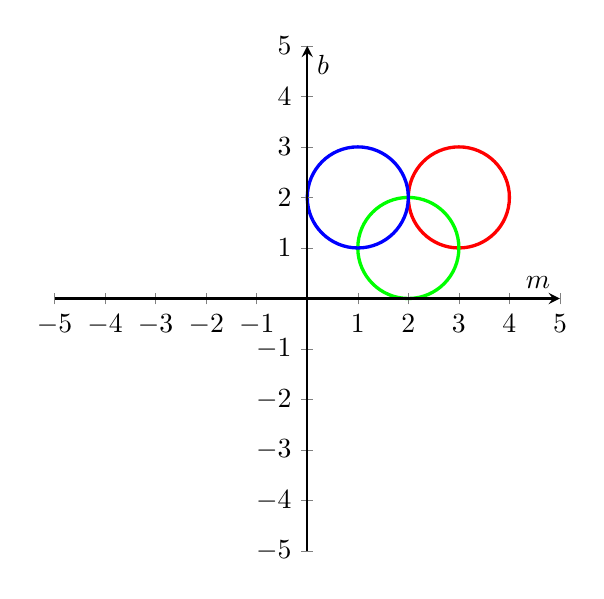
\begin{tikzpicture}
                        \begin{axis}[
                            axis on top=true,
                            axis line style=thick,
                            domain=-4:4, samples=9,
                            axis equal image,
                            axis lines=middle, xlabel=$m$, ylabel=$b$,
                            height=8cm, width=8cm,
                            enlargelimits=false,
                            xtick={-5,-4,...,5},
                            ytick={-5,-4,...,5},
                            xmin=-5, xmax=5,
                            ymin=-5, ymax=5
                        ]
                            \path (axis cs:0,0) coordinate (O);
                            \path (axis cs:1,0) coordinate (U);
                            \draw[very thick, red] let \p1=(O), \p2=(U), \n1={veclen(\x2-\x1,\y2-\y1)} in (axis cs:3,2) circle [radius=\n1];
                            \draw[very thick, green] let \p1=(O), \p2=(U), \n1={veclen(\x2-\x1,\y2-\y1)} in (axis cs:2,1) circle [radius=\n1];
                            \draw[very thick, blue] let \p1=(O), \p2=(U), \n1={veclen(\x2-\x1,\y2-\y1)} in (axis cs:1,2) circle [radius=\n1];
                        \end{axis}
                    \end{tikzpicture}
                    \hfill \phantom{}
                \end{center}
                If we don't know the radius, we set a range $r \in [r_\text{min}, r_\text{max}]$, and then perform a similar algorithm to before.
                \medskip

                Another representation of a circle can be done with trigonometric functions (parametric form);
                \begin{align*}
                    x & = a + r \cos \theta \\
                    y & = b + r \sin \theta
                \end{align*}
                However, if we know $\theta$, we can vote along a direction.
                Since we know the direction of an edge point (obtained from edge detection), we can narrow it down (along the gradient or opposite the gradient).
                We assume an accuracy of $\pm \phi$, and vote within that area.
                \begin{center}
                    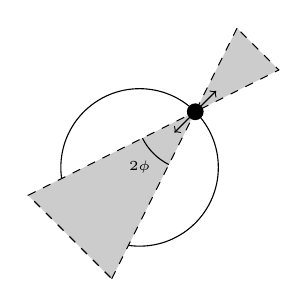
\begin{tikzpicture}
                        \draw (0, 0) circle (1);
                        \begin{scope}[shift={(0.707, 0.707)}, rotate={45}, scale={0.75}]
                            \draw[dashed, fill=black!20]
                            (1.5, 0.5) -- (0, 0) -- (1.5, -0.5) -- cycle
                            (-3, -1) -- (0, 0) -- (-3, 1) -- cycle;
                            \node[rbtb] at (0, 0) {};
                            \draw (0.5, 0) edge[<->] (-0.5, 0);
                            \draw (0, 0) ++(161.6:1) arc (161.6:198.4:1);
                        \end{scope}
                        \node at (0, 0) {\tiny $2 \phi$};
                    \end{tikzpicture}
                \end{center}
                The algorithm can be done as follows;
                \begin{enumerate}[1.]
                    \itemsep0em
                    \item initialise all bins $H(a, b, r)$ to zero
                    \item for each possible radius $r \in [r_\text{min}, r_\text{max}]$
                        \begin{enumerate}[a.]
                            \itemsep0em
                            \item for each edge point $(x, y)$;
                                \begin{enumerate}[i.]
                                    \itemsep0em
                                    \item let $\theta$ be gradient direction / opposite gradient direction
                                    \item calculate $a = x - r\cos \theta$ and $b = y - r\sin \theta$
                                    \item accumulate $H(a, b, r) = H(a, b, r) + 1$
                                \end{enumerate}
                        \end{enumerate}
                    \item find $(a, b, r)$ where $H(a, b, r)$ is a local maximum and larger than a threshold
                \end{enumerate}
\end{document}